\section{User Groups}
\begin{itemize}
\item Compose Workbench configurator: Developer who creates an Application with the help of the Compose Workbench.
\item Compose Workbench user: User of the application created by the Compose Workbench configurator.
\item Compose Workbench contributor: Developer which contributes towards the Compose Workbench.
\end{itemize}


\section{Compose Workbench Elements}
\subsection{Workbench}
The term Workbench is used to describe the complete application which is built by using the Compose Workbench Library.

\subsection{Module}
A Module represents a displayable element inside the workbench. It can be displayed as a Tab or Window and builds the interface to the workbench. Explorer and Editor are the two types of Modules. 

A Module provides following callback which will expose the Modules internal Model.
\begin{itemize}
    \item onClose: will be called when displayed element is closed.
    \item onSave: will be called when global save from Workbench is called.
\end{itemize}

\subsubsection{Explorer}
An Explorer is a type of Module which is used to Explore data. An Explorer can not be requested from outside the library. As best practice all data in an Explorer should be read only.

\subsubsection{Editor}
An Editor is a type of Module which is used to edit data. Editors can be requested by the Compose Workbench configurator from outside the library. This allows editing dynamic data which is displayed in an Explorer. To request an Editor the Controller of the editable Data must be provided.

\section{UI Elements}

\subsection{Main Window}
Main Workbench View refers to the initial Window which is opened when starting the Application. There ca be only one Instance of the Main Window at any time.

\begin{figure}[H]
    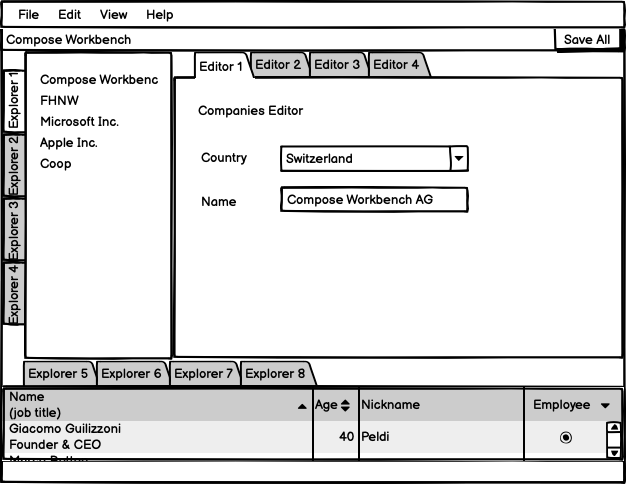
\includegraphics[width=1\linewidth]{images/WorkbenchCompose.png}
    \caption{Overview Main Window}
\end{figure}


The Main Window provides this Actions:
\begin{itemize}
    \item \textbf{Save All}: Sends a save request to all opened Editors.
    \item \textbf{Close}: Closes the Application.
    \item \textbf{Menu Bar}: Workbench specific and Configurator defined Actions are provided.
    \item \textbf{Workbench Menu}: Internal Menu as extension to Menu Bar. Where the Workbench Menu is mention to provide Application specific Actions.
\end{itemize}

\subsection{Tab}
A Tab displays the content of one Module inside the Main Window.

A Tab provides this Actions:
\begin{itemize}
    \item Drag and Drop: Tab can be dragged out of the main Window and dropped into a new Window.
    \item Close: Closes the Tab.
\end{itemize}

\begin{figure}[H]
\centering
\begin{subfigure}{.5\textwidth}
  \centering
  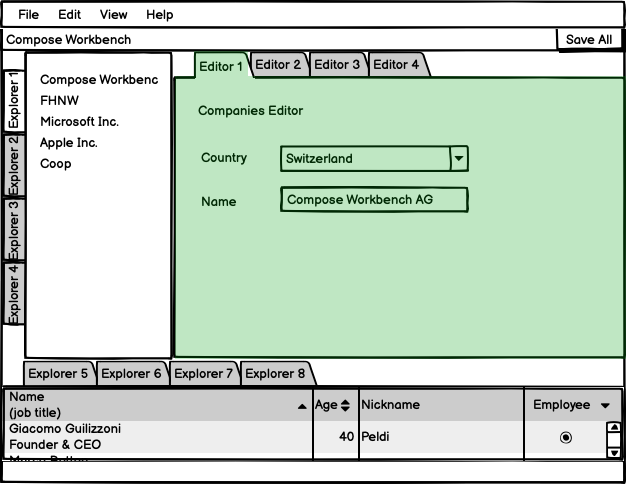
\includegraphics[width=.9\linewidth]{images/WorkbenchCompose (TabToWindow0) (TabToWindow0).png}
  \caption{Drag Tab on TabHeader}
  \label{fig:ransac_result}
\end{subfigure}%
\begin{subfigure}{.5\textwidth}
  \centering
  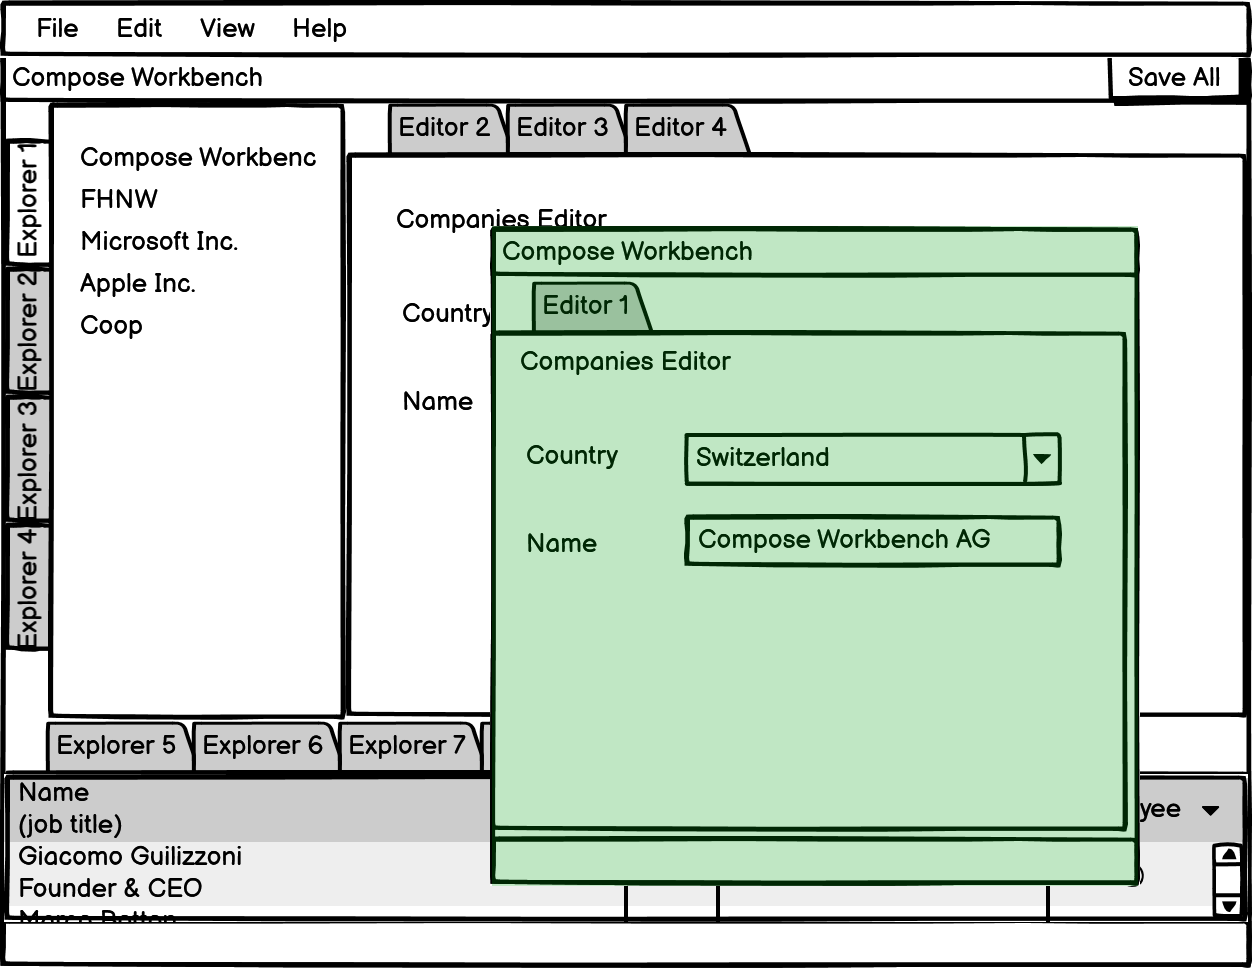
\includegraphics[width=.9\linewidth]{images/WorkbenchCompose (TabToWindow) (TabToWindow).png}
  \caption{Tab is moved out as separate Window}
  \label{fig:ransac_rotation}
\end{subfigure}
\caption{Drag and Drop for Tab/Window}
\label{fig:ransac_results}
\end{figure}

\subsection{Window}
A Window displays the content of one or more Modules outside the Main Window. There can be multiple Windows at the same time, the number of open windows is not limited.


A Window provides this Actions:
\begin{itemize}
    \item Drag: Module from the Window can be dragged back into the main Window or another open Window.
    \item Drop: Module from the main Window can be dropped into the Window
    \item Close: Closes the Window.
\end{itemize}

\subsection{Spaces}
The Workbench Main Window separates two kind of spaces, Editor Space and Explorer Space
\begin{figure}[H]
    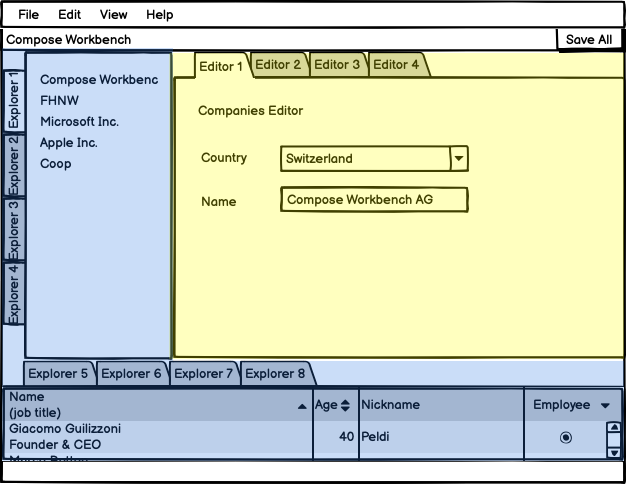
\includegraphics[width=1\linewidth]{images/WorkbenchCompose (SpacesColored) (SpacesColored).png}
    \caption{Editor Space (yellow), Explorer Space, (blue)}
\end{figure}

\subsubsection{Editor Space}


The Editor space displays all opened Editors as Tabs inside of the main Window. The Editor Space can be split once vertically or horizontally to display Editors next to each other. Editors can be moved from one to another split section by Drag and Drop.

\begin{figure}[H]
\centering
\begin{subfigure}{.5\textwidth}
  \centering
  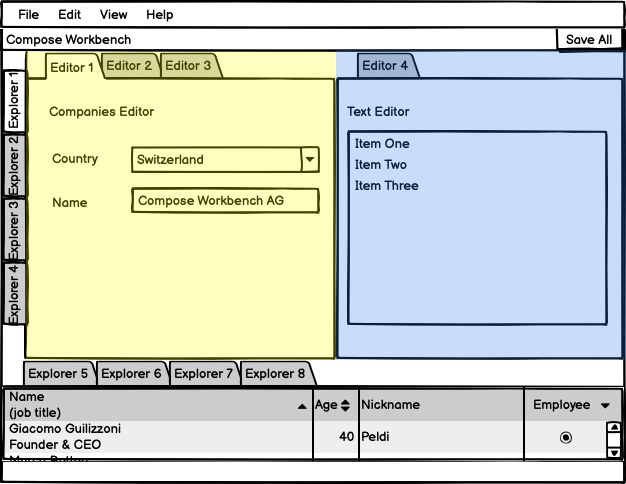
\includegraphics[width=.9\linewidth]{images/WorkbenchCompose (EditorSpaceVerticalSplit) (EditorSpaceVerticalSplit).png}
  \caption{Vertical Split View}
  \label{fig:ransac_result}
\end{subfigure}%
\begin{subfigure}{.5\textwidth}
  \centering
  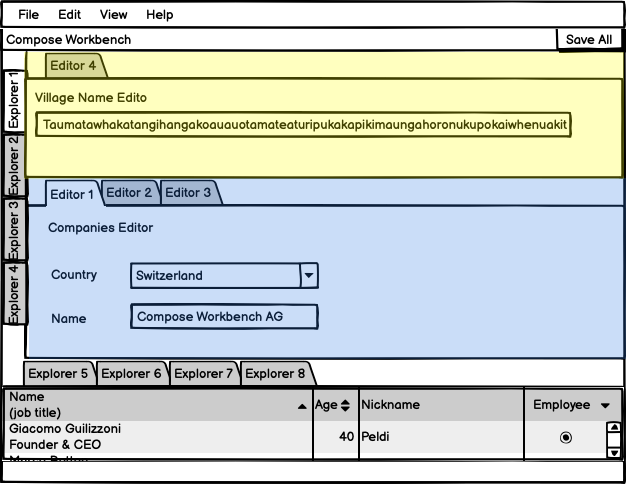
\includegraphics[width=.85\linewidth]{images/WorkbenchCompose (EditorSpaceHorizontalSplit) (EditorSpaceHorizontalSplit).png}
  \caption{Horizontal Split View}
  \label{fig:ransac_rotation}
\end{subfigure}
\caption{Split View on Editor Space}
\label{fig:ransac_results}
\end{figure}


\subsubsection{Explorer Space}

The Explorer space displays all opened Explorers as Tabs. The Explorer Tabs live inside Drawers which can be collapsed. The Explorer space is split into different drawers which have fixed positions (left and bottom). Explorers can be moved from one Drawer to another by Drag and Drop. 

\begin{figure}[H]
\centering
\begin{subfigure}{.5\textwidth}
  \centering
  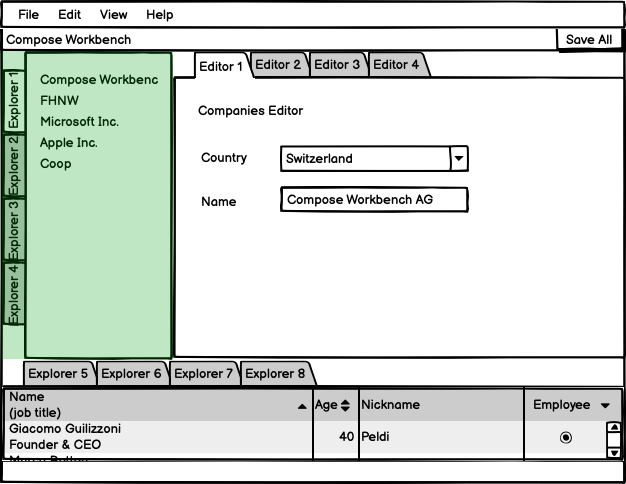
\includegraphics[width=.9\linewidth]{images/WorkbenchCompose (ExplorerSpaceCollapsed0) (ExplorerSpaceCollapsed0).png}
  \caption{Explorer Space open}
  \label{fig:ransac_result}
\end{subfigure}%
\begin{subfigure}{.5\textwidth}
  \centering
  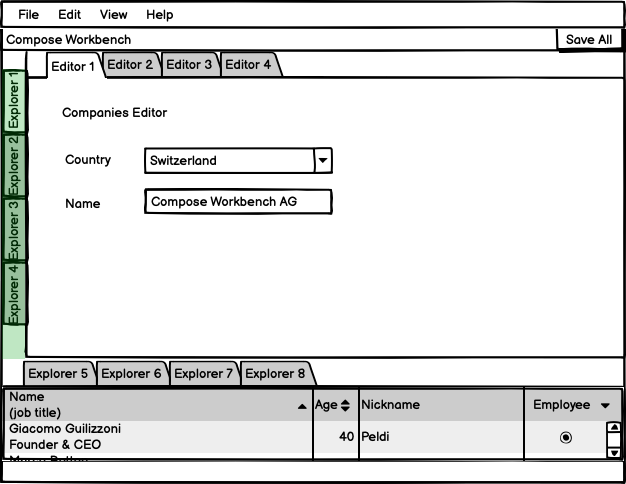
\includegraphics[width=.9\linewidth]{images/WorkbenchCompose (ExplorerSpaceCollapsed) (ExplorerSpaceCollapsed).png}
  \caption{Explorer Space collapsed}
  \label{fig:ransac_rotation}
\end{subfigure}
\caption{Collapsible Explorer Space}
\label{fig:ransac_results}
\end{figure}

\section{Subscribe and Update}
To allow communication between the Workbench Modules, the Workbench supports a topic base subscription and update mechanism. A Module can subscribe to a user defined topic and send updates on user defined topic. The Workbench will come with a set of predefined topics to use.

This mechanism can be used for example to notify about changes done in a editor or to notify about the closing of a editor or explorer.
